 \documentclass{beamer}
\usepackage{graphicx}
\usetheme{Warsaw}
\title{\textbf{Moogle} (Proyecto de Pogramación I)}
\author{Laura Alonso Rivero C-122}
\date{}
\usetheme{Warsaw}
\begin{document}
\maketitle
\begin{frame}
\begin{center}
\Large{¿Qué es Moogle?}\linebreak \\
\large{Es una  una aplicación web capaz de encontrar un texto en un
conjunto de documentos}\linebreak \\
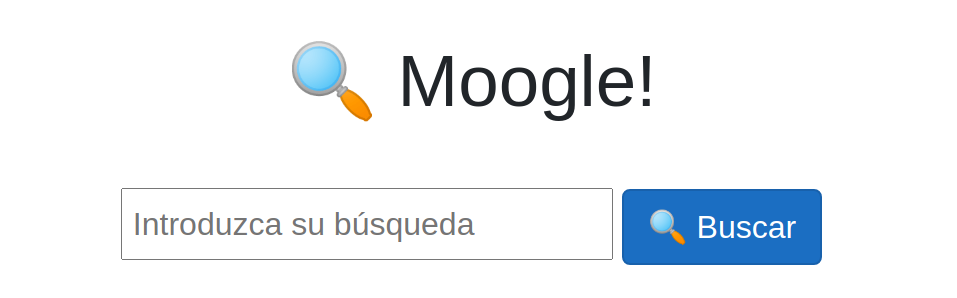
\includegraphics[width=7cm]{moogle.png}
\end{center}
\end{frame}

\begin{frame}
 \begin{flushleft}
\Large{El proyecto está estructurado de la siguiente manera:}
\begin{itemize}
\item\normalsize{Diccionario de palabras (palabra, Diccionario de documentos (docId, DetallesDelDocumento-palabra))}
\item\normalsize{DetallesDelDocumento-palabra [número de ocurrencias de la palabra en el documento, TF-IDF de la palabra en el documento]}
\item\normalsize{Doc [id de la ruta, nombre del documento, numero de palabras del documento]}
\item\normalsize{DirectoryName [id de la ruta, ruta completa del documento]}
\item\normalsize{Diccionario de Documentos (docId, Doc)}
\end{itemize}
\end{flushleft}
\end{frame}

\begin{frame}
 \begin{flushleft}
\Large{La carga de datos}\linebreak \\
\normalsize{Los datos son obtenidos a partir de los documentos que se encuentran en la carpeta \textbf{\textit{`Content`}} y a partir del método \textbf{\textit{`Initialize`}} se cargará la base de datos. \linebreak \\
Para cada fichero que se lea se procede a llenar el diccionario \textbf{\textit{`wordsDictionary`}} , los valores para esta llave serán otro diccionario llamado \textbf{\textit{`docsDictionary`}} donde se encuentra el \textbf{TF-IDF} de la palabra en el documento.}
\end{flushleft}
\end{frame}

\begin{frame}
 \begin{flushleft}
\Large{\textbf{TF-IDF (Term Frequency - Inverse Document Frecuency)}}
\end{flushleft}
\begin{center}
\begin{equation}
TF-IDF = \frac{\textup{cant de apariciones}}{\textup{cant de palabras}}\times\log\frac{\textup{total de docs}}{\textup{docs con la palabra}}
\end{equation}
\end{center}
\end{frame}

\begin{frame}
 \begin{flushleft}
\Large {\textbf{Búsqueda de palabras}}\linebreak \\
\large {Al iniciar la búsqueda el usuario puede elegir una palabra o una frase e incluir en cada palabra operadores tales como:}

\begin{itemize}
\item\large{ `\textexclamdown` (exige que la palabra no se encuentre en los documentos devueltos)}
\item\large{`\^` (exige que la palabra se encuentre en los documentos devueltos)
}
\item\large{`*` (da mayor importancia a los documentos que contengan esta palabra)
}
\end{itemize}
\end{flushleft}
\end{frame}

\begin{frame}
 \begin{flushleft}
\Large {Casos de usos erróneos:}

\begin{itemize}
\item\large{ Si la palabra contiene `\textexclamdown` como primer carácter y después le siguen otros operadores}
\item\large{Si la palabra contiene `\^` como primer carácter y después le siguen otros operadores}
\item\large{Si la palabra contiene `*` y después le sigue `\textexclamdown`}
\end{itemize}

\end{flushleft}
\end{frame}

\begin{frame}
 \begin{flushleft}
\large{Si se encuentra que alguna palabra contiene `\textexclamdown` se eliminan de la lista de búsqueda todos los documentos que la contengan. En cambio, si la palabra posee `\^` se eliminan todos los documentos que no la contengan}
\end{flushleft}
\end{frame}

\begin{frame}
 \begin{flushleft}
\large{Con estas palabras se procederá a llenar la lista \textbf{\textit{`results`}}  que devolverá los nombres de los documentos que contengan una o más de estas y los oredenará según  el valor del \textit{ TF-IDF}}
\end{flushleft}
\end{frame}

\begin{frame}
 \begin{flushleft}
\large{En caso de que no se encuentre la palabra se llenará la lista \textbf{\textit{`suggestions`}} que buscará
por el método de \textbf{\textit{`FindSimilarities`}} las cuatro palabras presentes en el diccionario más similares a esta.\linebreak \\
 Este método utiliza el algoritmo de 
Levenshtein (utiliza matrices siendo las filas las letras de la palabra de la query y las 
columnas las letras de la palabra del diccionario) para dar este criterio de similaridad.}
\end{flushleft}
\end{frame}

\begin{frame}
 \begin{flushleft}
\Large {\textbf{ Propuestas para el mejoramiento de la web en el futuro}}\linebreak \\
\begin{itemize}
\item\large{ Se puede utilizar el algoritmo de Porter a la hora de hacer el diccionario de palabras 
pues con este se va a eliminar todos los sufijos tales como género, numero, persona, 
tiempos verbales, diminutivos... y se quedara solamente con las raíces de las palabras 
lo que reducirá el tamaño del diccionario y hará que la carga de la basa de datos y 
posterior búsqueda de la query sea más rápida y eficiente.}
\end{itemize}
\end{flushleft}
\end{frame}

\begin{frame}
 \begin{flushleft}
\Large {\textbf{ Propuestas para el mejoramiento de la web en el futuro}}\linebreak \\
\begin{itemize}
\item\large{ Se puede guardar la data en un fichero estructurado para ahorrar tiempo a la hora de 
inicializar y recalcularlo solo cada vez que se carguen otros ficheros en la carpeta 
\textbf{\textit{`Content`}}.}
\item\large{ Se puede realizar una búsqueda exacta de frase de más de dos palabras que estén 
entre comillas en el criterio de búsqueda.}
\end{itemize}
\end{flushleft}
\end{frame}

\begin{frame}
 \begin{center}
\LARGE{Gracias por su atención}
\end{center}
\end{frame}

\end{document}